\section{Et après ...}

La Figure \ref{fig:circuit_HO1_HO2} reprend donc l'entierté du circuit implémenté jusqu'ici.

\begin{figure}[h!]
    \centering
    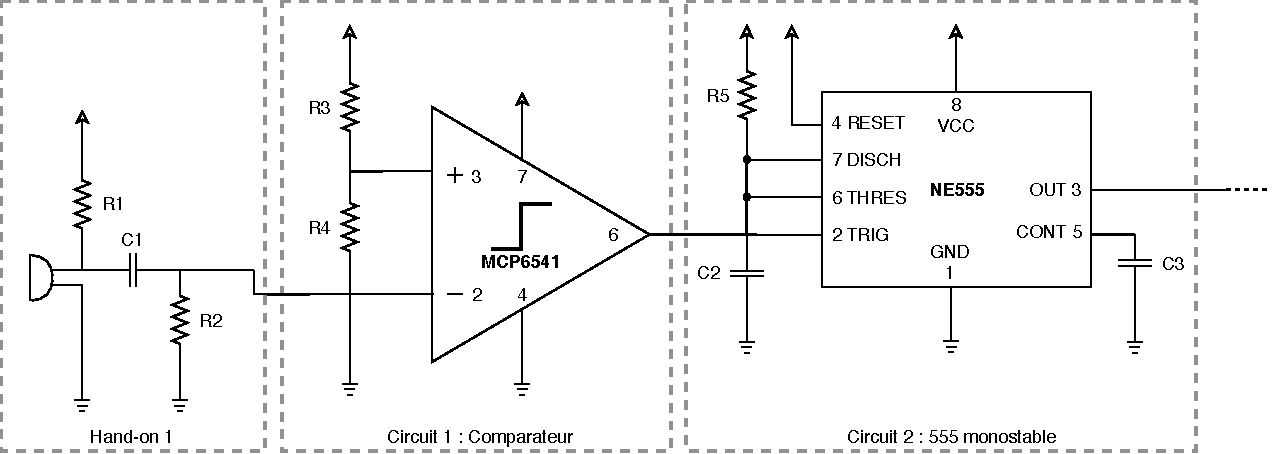
\includegraphics[width=1\linewidth]{HO1_HO2.pdf}
    \caption{Schéma du circuit HO1 et HO2.}
    \label{fig:circuit_HO1_HO2}
\end{figure}

Maintenant que nous disposons d'un signal bien défini à la sortie du \texttt{NE555}, nous sommes prêt à attaquer la dernière partie de ce projet, à savoir le circuit commandé. Nous vous proposons d'utiliser une lampe afin de pouvoir l'allumer et l'éteindre à distance, avec un simple claquement de doigt... mais bien d'autres applications sont possibles. Avez-vous d'autres idées ? N'hésite pas à nous les partager pour que l'on puisse discuter ensemble des détails un peu plus techniques ! Rendez-vous lundi prochain pour le dernier HO, bonne journée. Le \textsc{Club ELEC} :) 